\chapter{Architectural Smells and Refactorings}
\section{Definition}
A review of white and grey literature aimed at a determining the most recognised \textbf{architectural smells}\footnote{i.e. the \textit{"smell"} is caused by an \textbf{\textit{unproper}} architectural design choice} for \textit{microservices} and the architectural \textbf{refactorings} to resolve them.
In other terms, the problem is for a system designer to understand whether the designed infrastucture respects the microservices principles,
and, in case it doesn't, how to refactor it according to such principles.

\section{Design Principles}
\begin{enumerate}
   \item \textbf{Independent deployability}:
   Microservices forming an application should be indipendently deployable
   \item \textbf{Horizontal scalability}:
   They should also be horizontally scalable
   \item \textbf{Isolation of failures}:
   Failures should be isolated to avoid cascaded side-effects
   \item \textbf{Decentralization}:
   Decentralization should occur in all aspects of microservice-based applications,
   from data management to governance
\end{enumerate}

\begin{figure}[htbp]
   \centering
   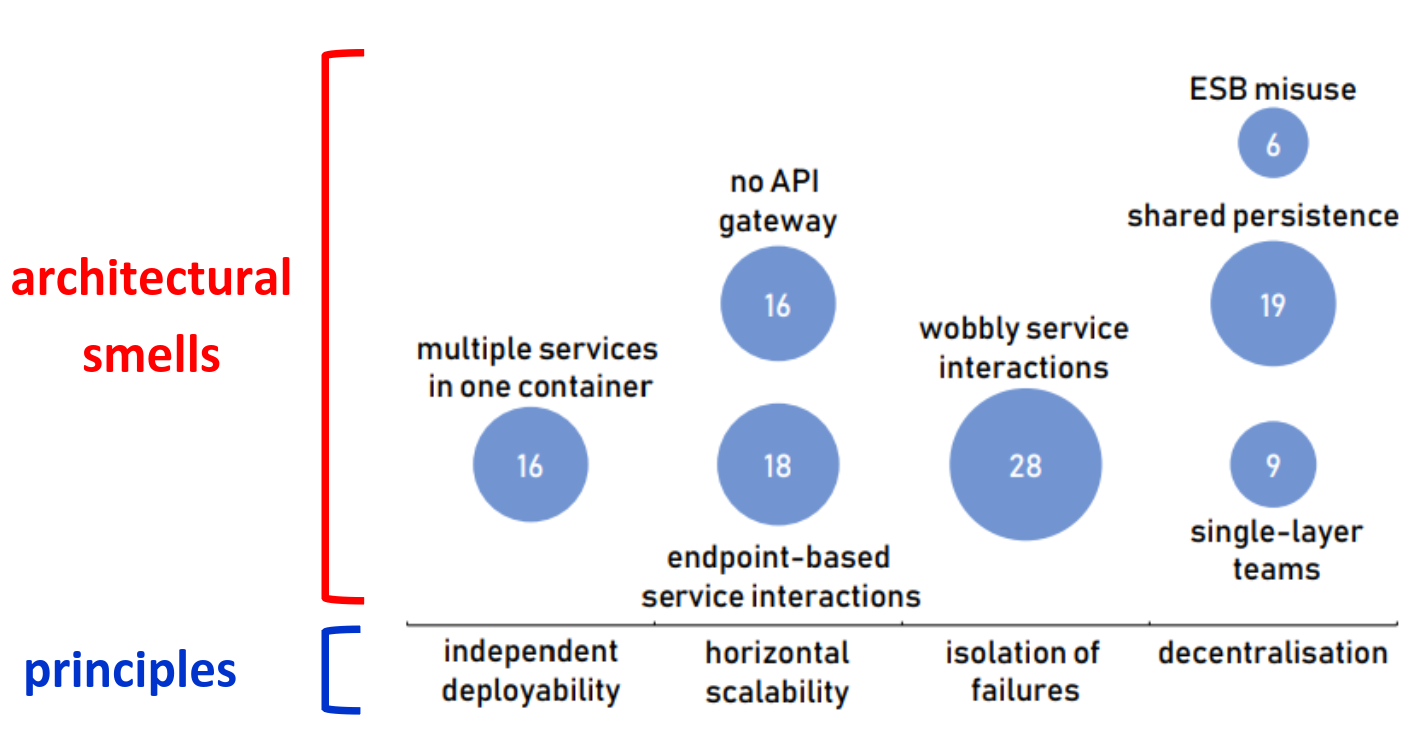
\includegraphics{images/smells_principles.png}
   \caption{Smells Principles}
   Here we can see smells, i.e. wrong choices, and the principle they violate
   \label{fig:smells_principles}
\end{figure}

\begin{figure}[htbp]
   \centering
   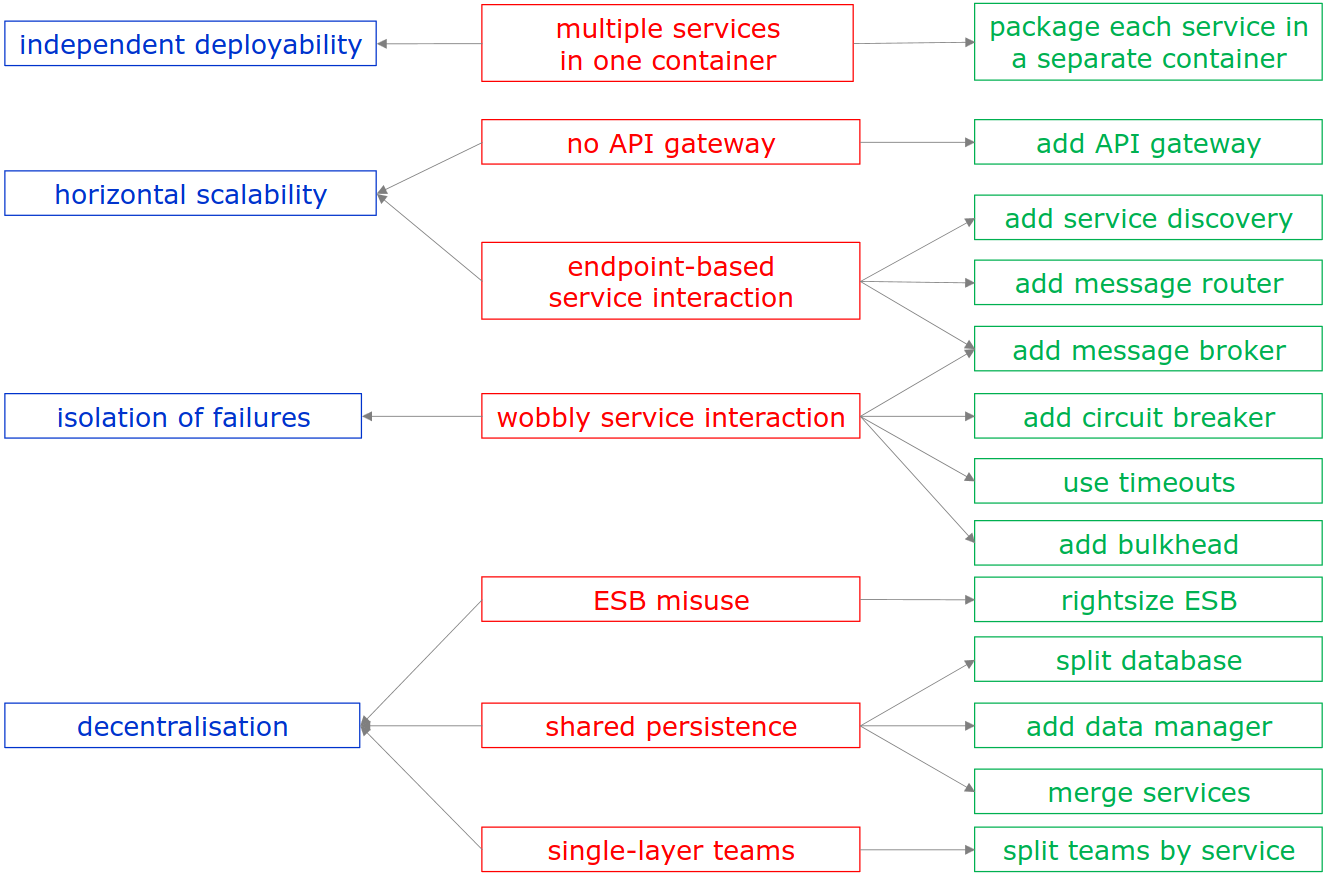
\includegraphics{images/smells_principles_solutions.png}
   \caption{Solutions}
   Here instead,
   we see also which are the design fixes we can implement to eliminate the bad smells.
   \label{fig:smells_principles_solutions}
\end{figure}


\begin{figure}[htbp]
   \centering
   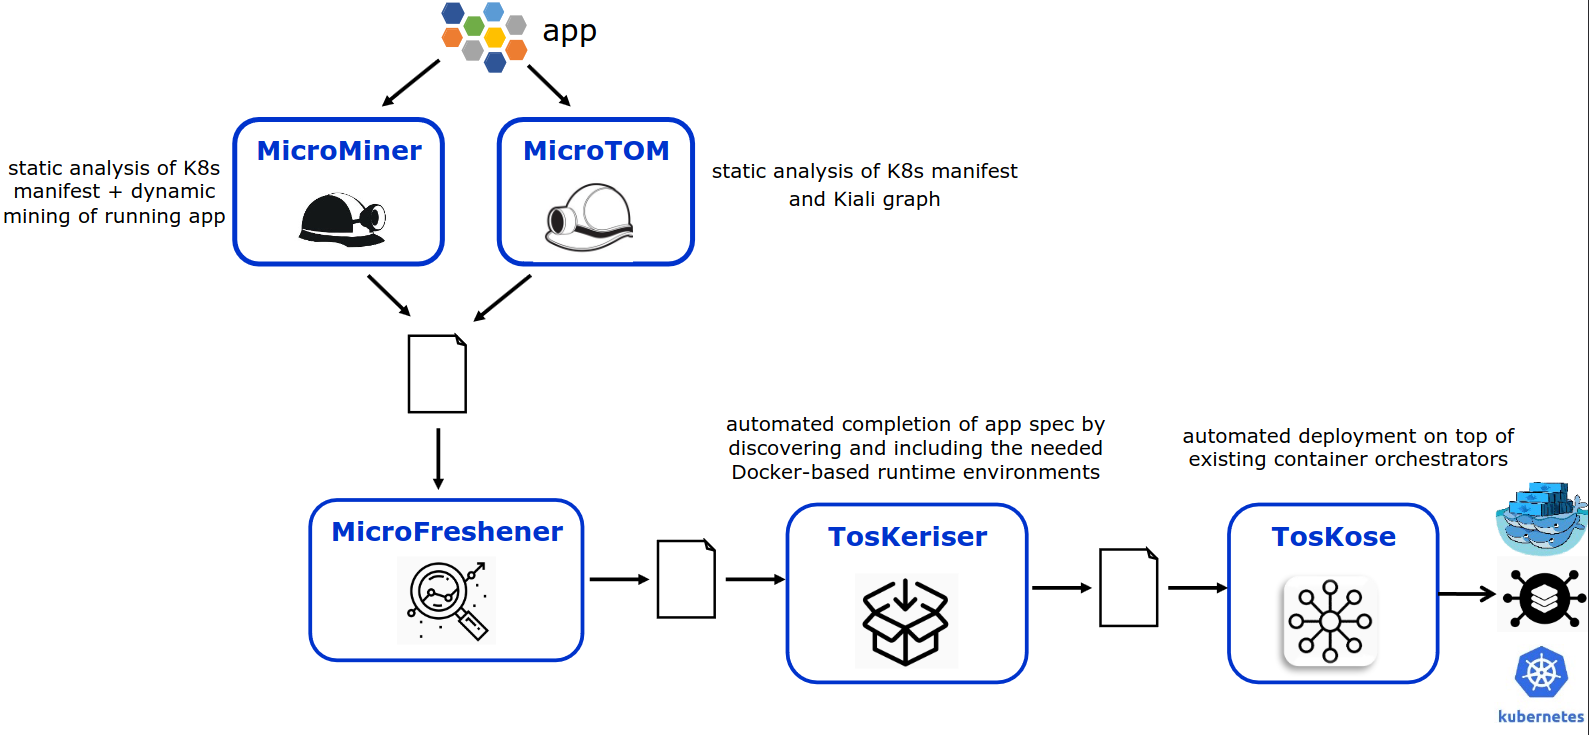
\includegraphics{images/microtoolchain.png}
   \caption{Microservices toolchain}
   \label{fig:microtoolchain}
\end{figure}